\documentclass[10pt]{beamer}

\usepackage[utf8]{inputenc}
\usepackage[english]{babel}
\usepackage{amssymb}
\usepackage{subfig}

\begin{document}

\begin{frame}{Computational Experiment: Visualizing Loss Function Convergence}
    \textbf{Goal of the experiment:} to assess how much the loss function changes when moving 
    from one training set size to the next:
    $$
    \Delta_k = \mathbb{E}_{p(\mathbf{w})} \bigl( \mathcal{L}_{k}(\mathbf{w}) - \mathcal{L}_{k-1}(\mathbf{w}) \bigr)^2
    $$
    where $\mathcal{L}$ is the loss function, $p(\mathbf{w})$ is a distribution, and $k$ is the dataset size index.

    \textbf{Method:} generate points according to $p(\mathbf{w})$ around the minimum point and 
    use Monte Carlo averaging.

    \begin{figure}[!htbp]
        \vspace*{-0.17cm}
        \centering
        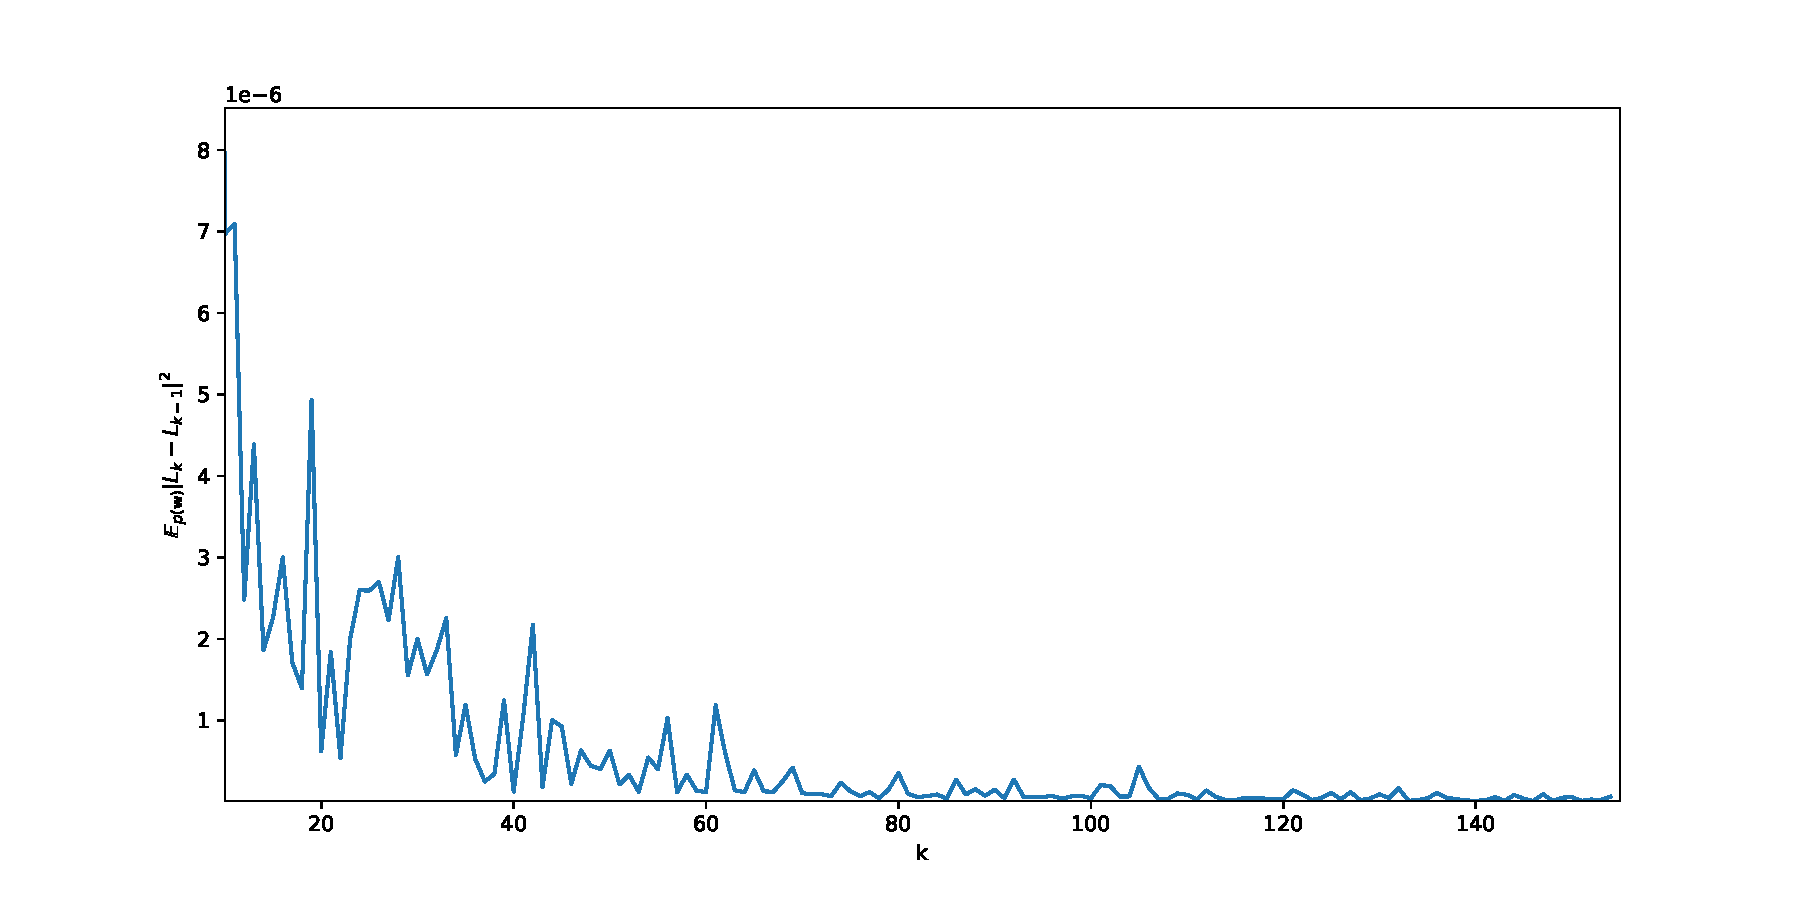
\includegraphics[width=0.82\textwidth]{img/Dm_32.pdf}
    \end{figure}
\end{frame}

\end{document}
